% !TEX root =  ../master.tex
\chapter{Nutzerhandbuch} %TODO: Das hier eventuell nochmal überarbeiten und kürzen?
Bei der Endwicklung der Anwendung haben wir großen Wert auf eine intuitive Gestaltung der \ac{GUI} und der \ac{UX} gelegt.
% TODO: ist das eine nicht-funktionale Anforderung?
Ziel war es, eine Anwendung zu gestalten, deren Nutzer die Anwendung ohne Erklärung verstehen.
Dennoch möchten wir in diesem Kapitel ein Referenzhandbuch erstellen.
In diesem Kapitel wird beschrieben, wie Nutzer die Anwendung verwenden können.

% TODO: Bilder müssen überall rein
\section{Öffnen der Anwendung}
Die Anwendung kann jederzeit \href{https://dhbwlearning.web.app}{\enquote{dhbwlearning.web.app}} geöffnet werden.
Wie jede andere Webapplikation kann dies über jedes Gerät, welches über eine Internetverbindung verfügt durch einen Webbrowser geöffnet werden.
Das heißt, die Anwendung steht den 24\,h pro Tag bereit und kann von allen Studenten und Dozenten verwendet werden.

\section{Login}
Nach dem Öffnen der Anwendung wird der Nutzer in der Regel aufgefordert sich einzuloggen.
In \autoref{fig:login} ist die Anmeldeseite dargestellt.

\begin{figure}[h]
    \centering
    \includegraphics[width=.7\textwidth]{img/Login}
    \caption{Login-Maske}
    \label{fig:login}
\end{figure}

Für die Anmeldung muss der Nutzer die Email-Adresse zu seinem Account, sowie das entsprechende Passwort angeben.
Setzt der Nutzer einen Hacken bei \enquote{Remember me}, so wird der Nutzer beim nächsten starten der Anwendung nicht um ein Password gebeten und wird automatisch in seinen Account eingeloggt.

Sollte der Nutzer noch keinen Account haben kann er auf \enquote{Register} klick, um sich selbst für die Nutzung der Anwendung zu registrieren.
Genaueres zur Registrierung sind in \autoref{sec:registrierung} beschrieben.

Sollte der Nutzer bereits einen Account haben und nur das Password zu diesem vergessen haben gibt es neben dem Password-Feld einen \enquote{Forgot Password?}-Button.
Dieser leitet den Nutzer zu einem Password-Vergessen-Formular weiter, welches in \autoref{sec:passwordVergessen} beschrieben ist.

Hat der Nutzer eine korrekte Email- und Passwordkombination eingetragen und auf \enquote{Login} geklickt, wird der Nutzer auf das Dashboard (vgl. \autoref{sec:dashboard}) weitergeleitet.
Andernfalls wird der Nutzer freundlich darauf hingewiesen, dass das Password nicht korrekt ist.



\section{Registrierung}\label{sec:registrierung}
Die Registrierungs-Maske dient dazu, einen neuen Nutzer in der Anwendung anzulegen.
Damit sich Nutzer registrieren können müssen sie eine Email-Adresse sowie ein Password wählen.
Der Nutzer kann hierbei eine beliebige, sogar eine Wegwerf-Email verwenden.
Die Email wird intern lediglich für Authentifizierungszwecke benötigt.
Das heißt die Email wird nur für das Login und für den Fall, dass ein Nutzer sein Passwort vergessen hat benötigt (vgl \autoref{sec:passwordVergessen}).
Verwendet der Nutzer eine Wegwerf-Email kann der die Anwendung wie gewohnt nutzen, verliert aber die Möglichkeit sein Passwort zurückzusetzen.

Das Password kann frei gewählt werden, solange es mindestens 6 und maximal 50 Zeichen hat.
Es gibt keine weiteren Einschränkungen, da wir der Meinung sind, dass aufwändige Passwortvorgaben eine schlechte \ac{UX} ergibt.
Dennoch sollten Nutzer Passwörter verwenden, die allgemein als sicher gelten.
% TODO: Vielleicht nochmal sagen, das wir sicher sind, weil firebase google auth?
Um zu verhindern, dass sich der Nutzer bei seinem Passwort vertippt hat, muss das Passwort ein zweites Mal bestätigt werden.

Schließlich muss der User den Nutzungsbedingungen zustimmen.
% TODO:

Sollte der Nutzer bereits einen Useraccount besitzen kann er jederzeit durch einen klick auf \enquote{Log in} zur Login-Maske zurückkehren.

Ist alles korrekt ausgefüllt kann der Nutzer durch klick auf \enquote{Registrieren} die Anmeldung abschließen und wird automatisch eingeloggt.

\begin{figure}[h]
    \centering
    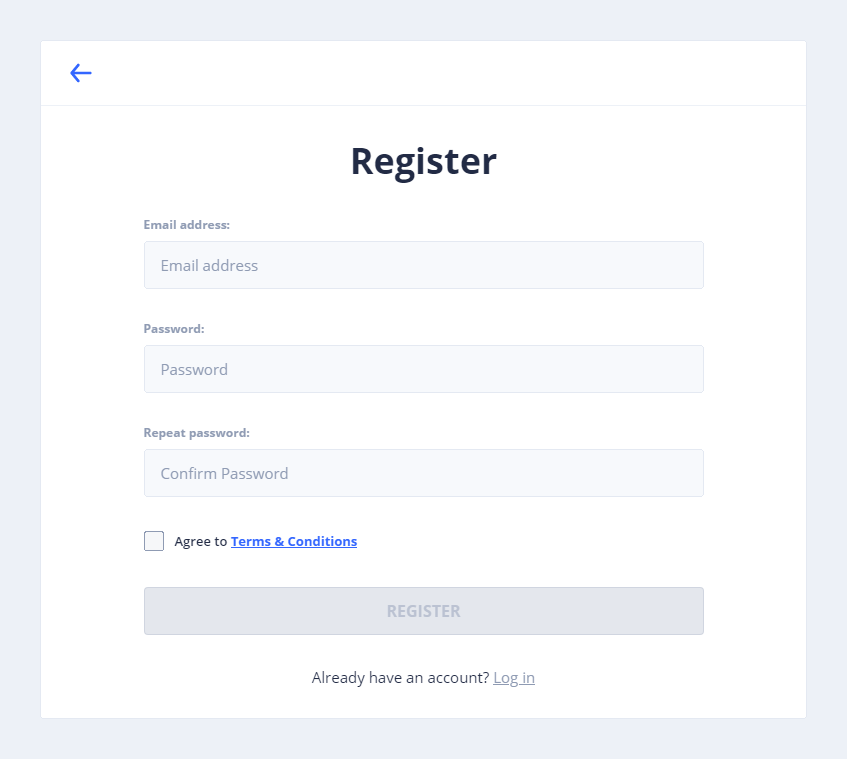
\includegraphics[width=.7\textwidth]{img/register.png}
    \caption{Registrierungs-Maske}
    \label{fig:registrierung}
\end{figure}


\section{Password-Vergessen}\label{sec:passwordVergessen}
Die Password-Vergessen-Funktion dient zum Zurücksetzen des Passwortes.
Möchte der Nutzer sein Password zurücksetzen und erneut Zugang zu seinem Account bekommen kann der Nutzer jederzeit seine Email in das Password-Vergessen-Feld eingeben.

\begin{figure}[h]
    \centering
    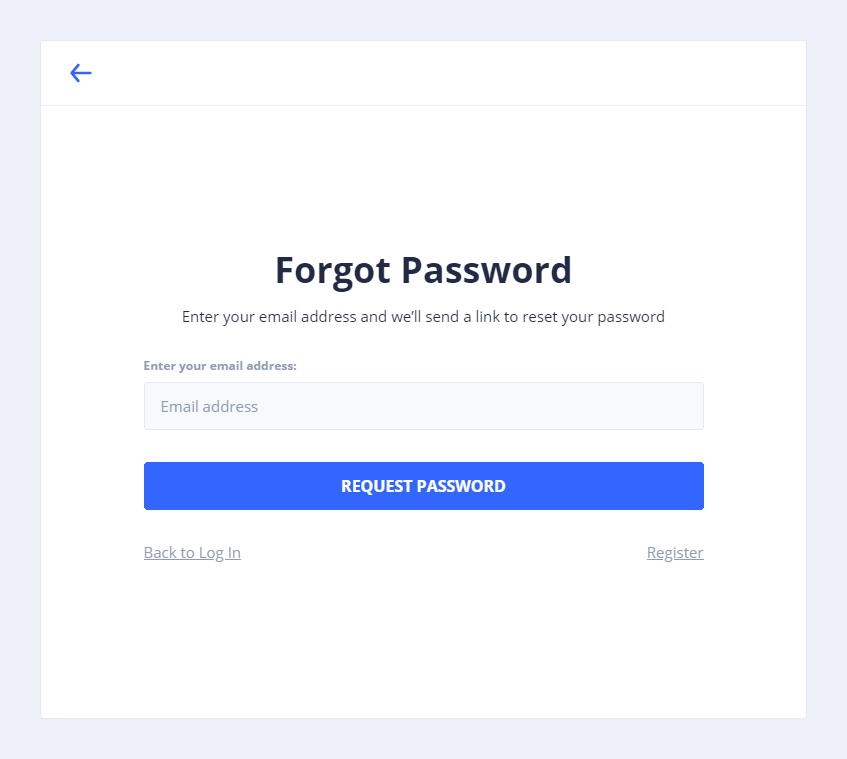
\includegraphics[width=.7\textwidth]{img/passwordReset.png}
    \caption{Password-Vergessen-Maske}
    \label{fig:passwordVergessen}
\end{figure}

Nachdem der Nutzer auf \enquote{Request Password} geklickt hat wird automatisch eine Email an die angegebene Email-Adresse gesendet.
Die Email enthält einen Link, mithilfe dem der Nutzer sein Passwort ändern kann.
Der Link leitet den Nutzer auf die in \autoref{fig:passwordVergessen} dargestellte Maske in der der Nutzer sein Passwort ändern kann.
Hat der Nutzer sein Passwort geändert wird der zu einem erneuten Login auf die Login-Maske geleitet.

Anzumerken ist, dass der Link zum Passwort ändern nur einmal gültig ist.
Sollte das Passwort bereits geändert worden sein, muss eine neue Email angefordert werden.
Dies verhindert, dass unberechtigte Personen die Email mitlesen können und das Passwort erneut ändern könn

% TODO: Muss man hier jede kleinigkeit schreiben? also das email auch wirklich eine email sein muss?


\begin{figure}[h]
    \centering
    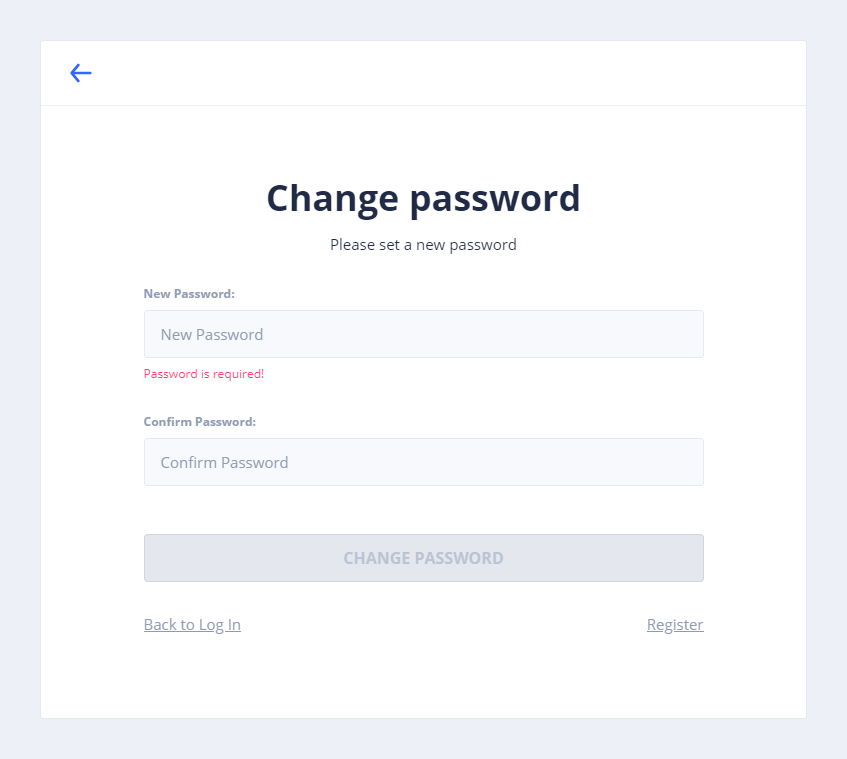
\includegraphics[width=.7\textwidth]{img/passwordReset2.png}
    \caption{Password-Aktualisieren-Maske}
    \label{fig:passwordVergessen2}
\end{figure}

% ..


\section{Dashboard}\label{sec:dashboard}
... siehe User Journey

% TODO: Das hier schreiben, wenn da tatsächlich was implementiert ist

